% Created 2024-02-20 mar 11:21
% Intended LaTeX compiler: pdflatex
\documentclass[aspectratio=169, usenames,svgnames,dvipsnames]{beamer}
\usepackage[utf8]{inputenc}
\usepackage[T1]{fontenc}
\usepackage{graphicx}
\usepackage{longtable}
\usepackage{wrapfig}
\usepackage{rotating}
\usepackage[normalem]{ulem}
\usepackage{amsmath}
\usepackage{amssymb}
\usepackage{capt-of}
\usepackage{hyperref}
\usepackage{color}
\usepackage{listings}
\usepackage{mathpazo}
\usepackage{gensymb}
\usepackage{amsmath}
\usepackage{diffcoeff}
\usepackage{steinmetz}
\usepackage{mathtools}
\usepackage{fancyvrb}
\DefineVerbatimEnvironment{verbatim}{Verbatim}{fontsize=\tiny, formatcom = {\color{black!70}}}
\bibliographystyle{plain}
\usepackage{siunitx}
\sisetup{per-mode=symbol}
\sisetup{output-decimal-marker={,}}
\DeclareSIUnit{\watthour}{Wh}
\DeclareSIUnit{\wattpeak}{Wp}
\DeclareSIUnit{\watthour}{Wh}
\DeclareSIUnit{\amperehour}{Ah}
\usepackage{steinmetz}
\hypersetup{colorlinks=true, linkcolor=Blue, urlcolor=Blue}
\usepackage[symbol, perpage]{footmisc}
\parskip=5pt
\usetheme{Boadilla}
\usecolortheme{rose}
\usefonttheme{serif}
\author{\href{https://oscarperpinan.github.io}{Oscar Perpiñán Lamigueiro}}
\date{}
\title{Configuración Eléctrica del Generador FV en un SFCR}
\subtitle{Energía Solar Fotovoltaica}
\institute[UPM]{Universidad Politécnica de Madrid}
\setbeamercolor{alerted text}{fg=blue!50!black} \setbeamerfont{alerted text}{series=\bfseries}
\AtBeginSubsection[]{\begin{frame}[plain]\tableofcontents[currentsubsection,sectionstyle=show/hide,subsectionstyle=show/shaded/hide]\end{frame}}
\AtBeginSection[]{\begin{frame}[plain]\tableofcontents[currentsection,hideallsubsections]\end{frame}}
\beamertemplatenavigationsymbolsempty
\setbeamertemplate{footline}[frame number]
\setbeamertemplate{itemize items}[triangle]
\setbeamertemplate{enumerate items}[circle]
\setbeamertemplate{section in toc}[circle]
\setbeamertemplate{subsection in toc}[circle]
\hypersetup{
 pdfauthor={\href{https://oscarperpinan.github.io}{Oscar Perpiñán Lamigueiro}},
 pdftitle={Configuración Eléctrica del Generador FV en un SFCR},
 pdfkeywords={},
 pdfsubject={},
 pdfcreator={Emacs 29.1 (Org mode 9.6.11)}, 
 pdflang={Spanish}}
\begin{document}

\maketitle

\section{Configuración Eléctrica del Generador}
\label{sec:org974d758}

\begin{frame}[label={sec:org74c45fd},plain]{}
\begin{center}
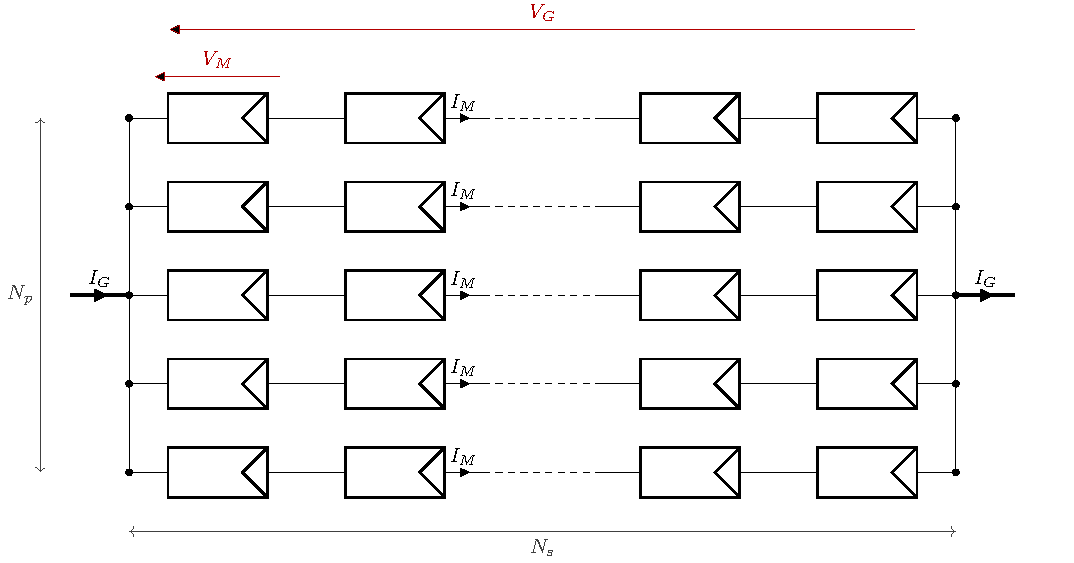
\includegraphics[height=0.9\textheight]{../figs/ConfiguracionGenerador.pdf}
\end{center}
\end{frame}

\begin{frame}[label={sec:org1628f9d},plain]{Planteamiento}
\begin{center}
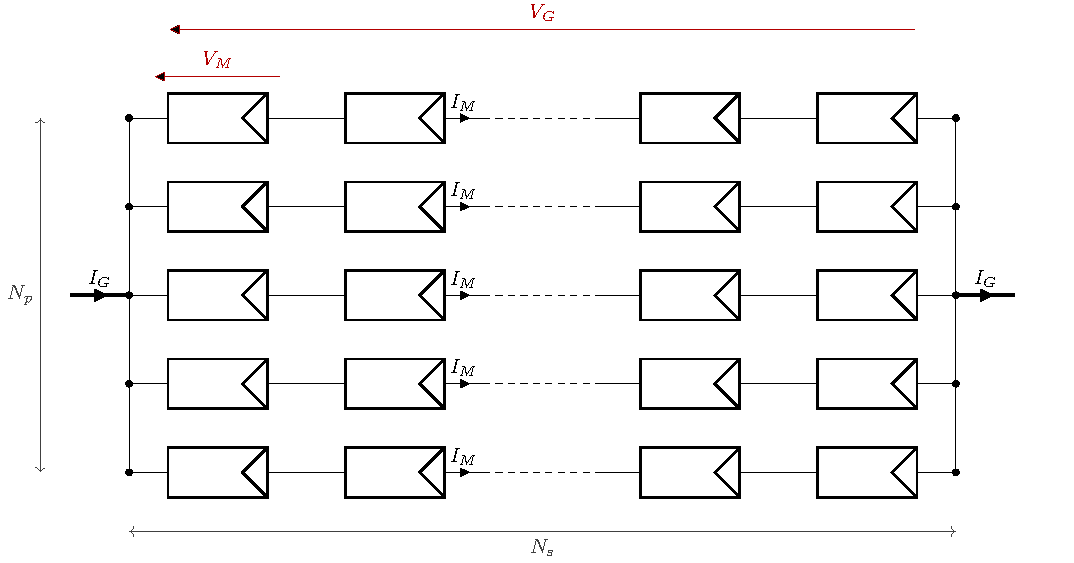
\includegraphics[height=0.5\textheight]{../figs/ConfiguracionGenerador.pdf}
\end{center}

\begin{itemize}
\item \alert{Objetivo}: determinar número de módulos en serie (\(N_s\)) y ramas en paralelo (\(N_p\)).
\item No tomamos en cuenta dispersión de parámetros: todos los módulos tienen la \alert{misma tensión} (\(V_M\)) y la \alert{misma corriente} (\(I_M\)).
\begin{align*}
  V_G &= N_S \cdot V_M\\
  I_G &= N_P \cdot I_M
\end{align*}
\end{itemize}
\end{frame}
\begin{frame}[label={sec:org2a19134}]{Modulos en serie}
\begin{itemize}
\item El inversor está diseñado para soportar una \alert{tensión máxima en la
entrada}, \(V_{max,inv}\).

Superarla puede conllevar la \alert{avería} del equipo.

\[
  \max(V_{ocG}) < V_{max,inv}
\]
\item El algoritmo de \alert{búsqueda del MPP} se realiza en un
rango de tensiones limitado, \(V_{mppMIN}, V_{mppMAX}\).

Para \alert{evitar pérdidas} por trabajar en un punto alejado del MPP, la tensión del generador debe estar dentro de este rango:

\[
  V_{mppMIN} \leq V_{mppG} \leq V_{mppMAX}
\]
\end{itemize}
\end{frame}
\begin{frame}[label={sec:org3245e3e}]{Procedimiento de cálculo}
\framesubtitle{Tensión máxima}

\begin{itemize}
\item Temperatura de célula (\(G=\qty{200}{\watt\per\meter\squared},\, T_{a}=\qty{-10}{\celsius}\))
\end{itemize}
\[
  T_{c} = T_{a} + G \cdot \frac{NOCT-20}{800} \rightarrow   T_{c} = -10 + 200 \cdot \frac{NOCT-20}{800}
\]

\begin{itemize}
\item Tensión del módulo
\end{itemize}
\[
  V_{ocM} = V_{ocM}^{*} + (T_{c}-T_{c}^{*})\cdot\frac{dV_{oc}}{dT_{c}} \rightarrow V_{ocM} = V_{ocM}^{*} + (T_{c}- 25)\cdot\frac{dV_{oc}}{dT_{c}}
\]
\begin{itemize}
\item Número de módulos en serie
\end{itemize}
\[
      V_{ocG} = N_s \cdot V_{ocM} \rightarrow N_{sMAX}=\frac{V_{max,inv}}{V_{ocM}}
\]
\end{frame}

\begin{frame}[label={sec:orgf17cfb2}]{Procedimiento de cálculo}
\framesubtitle{Tensión MPP}
\begin{itemize}
\item Temperatura de célula (\(G_{stc},\, T_{a}=\qty{25}{\celsius}\))
\end{itemize}
\[
  T_{c} = T_{a} + G \cdot \frac{NOCT-20}{800} \rightarrow T_{c} = 25 + 1000 \cdot \frac{NOCT-20}{800}
\]
\begin{itemize}
\item Tensión de circuito abierto del módulo
\end{itemize}
\[
  V_{ocM} = V_{ocM}^{*} + (T_{c}-T_{c}^{*})\cdot\frac{dV_{oc}}{dT_{c}} \rightarrow
  V_{ocM} = V_{ocM}^{*} + (T_{c}- 25)\cdot\frac{dV_{oc}}{dT_{c}}
\]
\end{frame}
\begin{frame}[label={sec:org80d62cc}]{Procedimiento de cálculo}
\framesubtitle{Tensión MPP}

\begin{itemize}
\item Tensión MPP del módulo
\end{itemize}
\[
  V_{mppM} = V_{ocM} \cdot \frac{V_{mppM}^*}{V_{ocM}^*}
\]
\begin{itemize}
\item Número de módulos en serie
\end{itemize}
\[
  V_{mppG} = N_s \cdot V_{mppM} \rightarrow
  \begin{cases}
    N_{sMPP}^{min} =\frac{V_{mppMIN}}{V_{mppM}}\\
    \\
    N_{sMPP}^{max} = \frac{V_{mppMAX}}{V_{mppM}}
  \end{cases}
\]
\end{frame}
\begin{frame}[label={sec:org51c8fb0}]{Ramas en paralelo}
\begin{itemize}
\item El fabricante del inversor elige los componentes para soportar una \alert{corriente máxima admisible}, \(I_{max,INV}\).

\item En general, el inversor es capaz de autoprotegerse ante valores superiores a este umbral desplazando el punto de funcionamiento del generador fuera del MPP.

\item No obstante, el diseñador del sistema debe elegir el número de ramas en paralelo de forma que no se supere este umbral.
\end{itemize}

\[
    N_{pMAX}=\frac{I_{max,INV}}{I_{scM}^{*}}
\]
\end{frame}

\begin{frame}[label={sec:orgfd1ab2b}]{Configuración del generador}
De los cálculos anteriores se obtiene un \alert{conjunto de configuraciones} del generador que permiten un buen acoplamiento entre inversor y generador. 

Para \alert{elegir una configuración} deben tenerse en cuenta diferentes aspectos:

\begin{itemize}
\item Configuración eléctrica y ubicación física de los módulos en la
estructura.

\item Inversión y rendimiento económicos.

\item Espacio disponible.

\item Relación de potencias de generador e inversor.

\item La curva de eficiencia del inversor depende de la tensión de entrada.
\end{itemize}
\end{frame}

\begin{frame}[label={sec:orge0826a1}]{Configuración eléctrica y estructura}
\begin{itemize}
\item Es recomendable elegir \alert{series} compuestas por un número de módulos
que puedan ser ubicados en una \alert{única hilera de la estructura}.

\begin{itemize}
\item \alert{Se facilita el trazado del cableado}:

La propia estructura puede servir como fijación auxiliar, se
evitan cruzamientos indeseados.

\item \alert{Se minimiza la influencia de las sombras}:

Es muy frecuente la aparición de sombras entre partes del
generador o entre seguidores, sombras de forma rectangular y que
comienzan afectando a las partes bajas de la estructura. Al
cablear por hileras, las sombras de las hileras bajas no afectan
a las hileras inmediatamente superiores.
\end{itemize}
\end{itemize}
\end{frame}

\begin{frame}[label={sec:org750e93d}]{Inversión y rendimiento económicos}
\begin{itemize}
\item La potencia del generador fotovoltaico está relacionada directamente
con la \alert{inversión económica} a realizar.

\item Por otra parte, la relación entre \alert{energía generada} y potencia
nominal es aproximadamente lineal, y por tanto, los \alert{ingresos
económicos} dependen casi linealmente de la potencia del generador.

\item Por tanto, para decidir la potencia del generador
(\(P_{g}^{*}=N_{s}\cdot N_{p}\cdot P_{m}^{*}\)) debe tenerse en cuenta
el capital o financiación disponible, y el rendimiento económico
deseado.
\end{itemize}
\end{frame}

\begin{frame}[label={sec:orgda628fc}]{Terreno ocupado}
\begin{itemize}
\item La potencia del generador es proporcional al área del generador y al \alert{terreno ocupado} (que también influye, aunque en menor grado, en el cálculo económico).

\item Por tanto, debe tenerse en cuenta el espacio disponible (o el coste que se pretende asumir por el uso de terreno).
\end{itemize}
\end{frame}

\begin{frame}[label={sec:orgb510c90}]{Relación de potencias entre generador e inversor}
Dado que la potencia entregada por el generador varía con las condiciones meteorológicas, el inversor trabajará en diferentes zonas de su curva de eficiencia.

\begin{center}
\includegraphics[height=0.75\textheight]{../figs/CurvaInversor.pdf}
\end{center}
\end{frame}


\begin{frame}[label={sec:org830ae96}]{Relación de potencias entre generador e inversor}
\begin{itemize}
\item Por tanto, una de las preguntas a responder es \alert{qué relación debe existir entre la potencia del generador FV y el inversor}.
\end{itemize}

\[
  F_{DI} = P_{g}^{*}/P_{inv}
\]

\begin{itemize}
\item Si esta relación es alta, el inversor trabajará con frecuencia en la región de alta eficiencia, pero a cambio es posible que deba limitar la potencia del generador para evitar superar su umbral de corriente admisible.
\end{itemize}
\end{frame}

\begin{frame}[label={sec:orge1ea6e9}]{Relación de potencias entre generador e inversor}
\begin{itemize}
\item Según el \alert{tipo de sistema} (estático, seguimiento) se debe elegir una relación de potencias de generador e inversor.

\item En \alert{sistemas de seguimiento} esta probabilidad suele ser alta. Se recomiendan inversores de potencia similar a la del generador  (\(P_{g}^{*}/P_{inv}\in\left[1;1.2\right]\))

\item No obstante, es posible demostrar que el valor de esta relación no es tan crítico como \alert{elegir un inversor con buena curva de eficiencia}.
\end{itemize}
\end{frame}

\section{Cableado Eléctrico}
\label{sec:org49e8e66}

\begin{frame}[label={sec:org68c101d},plain]{}
\begin{center}
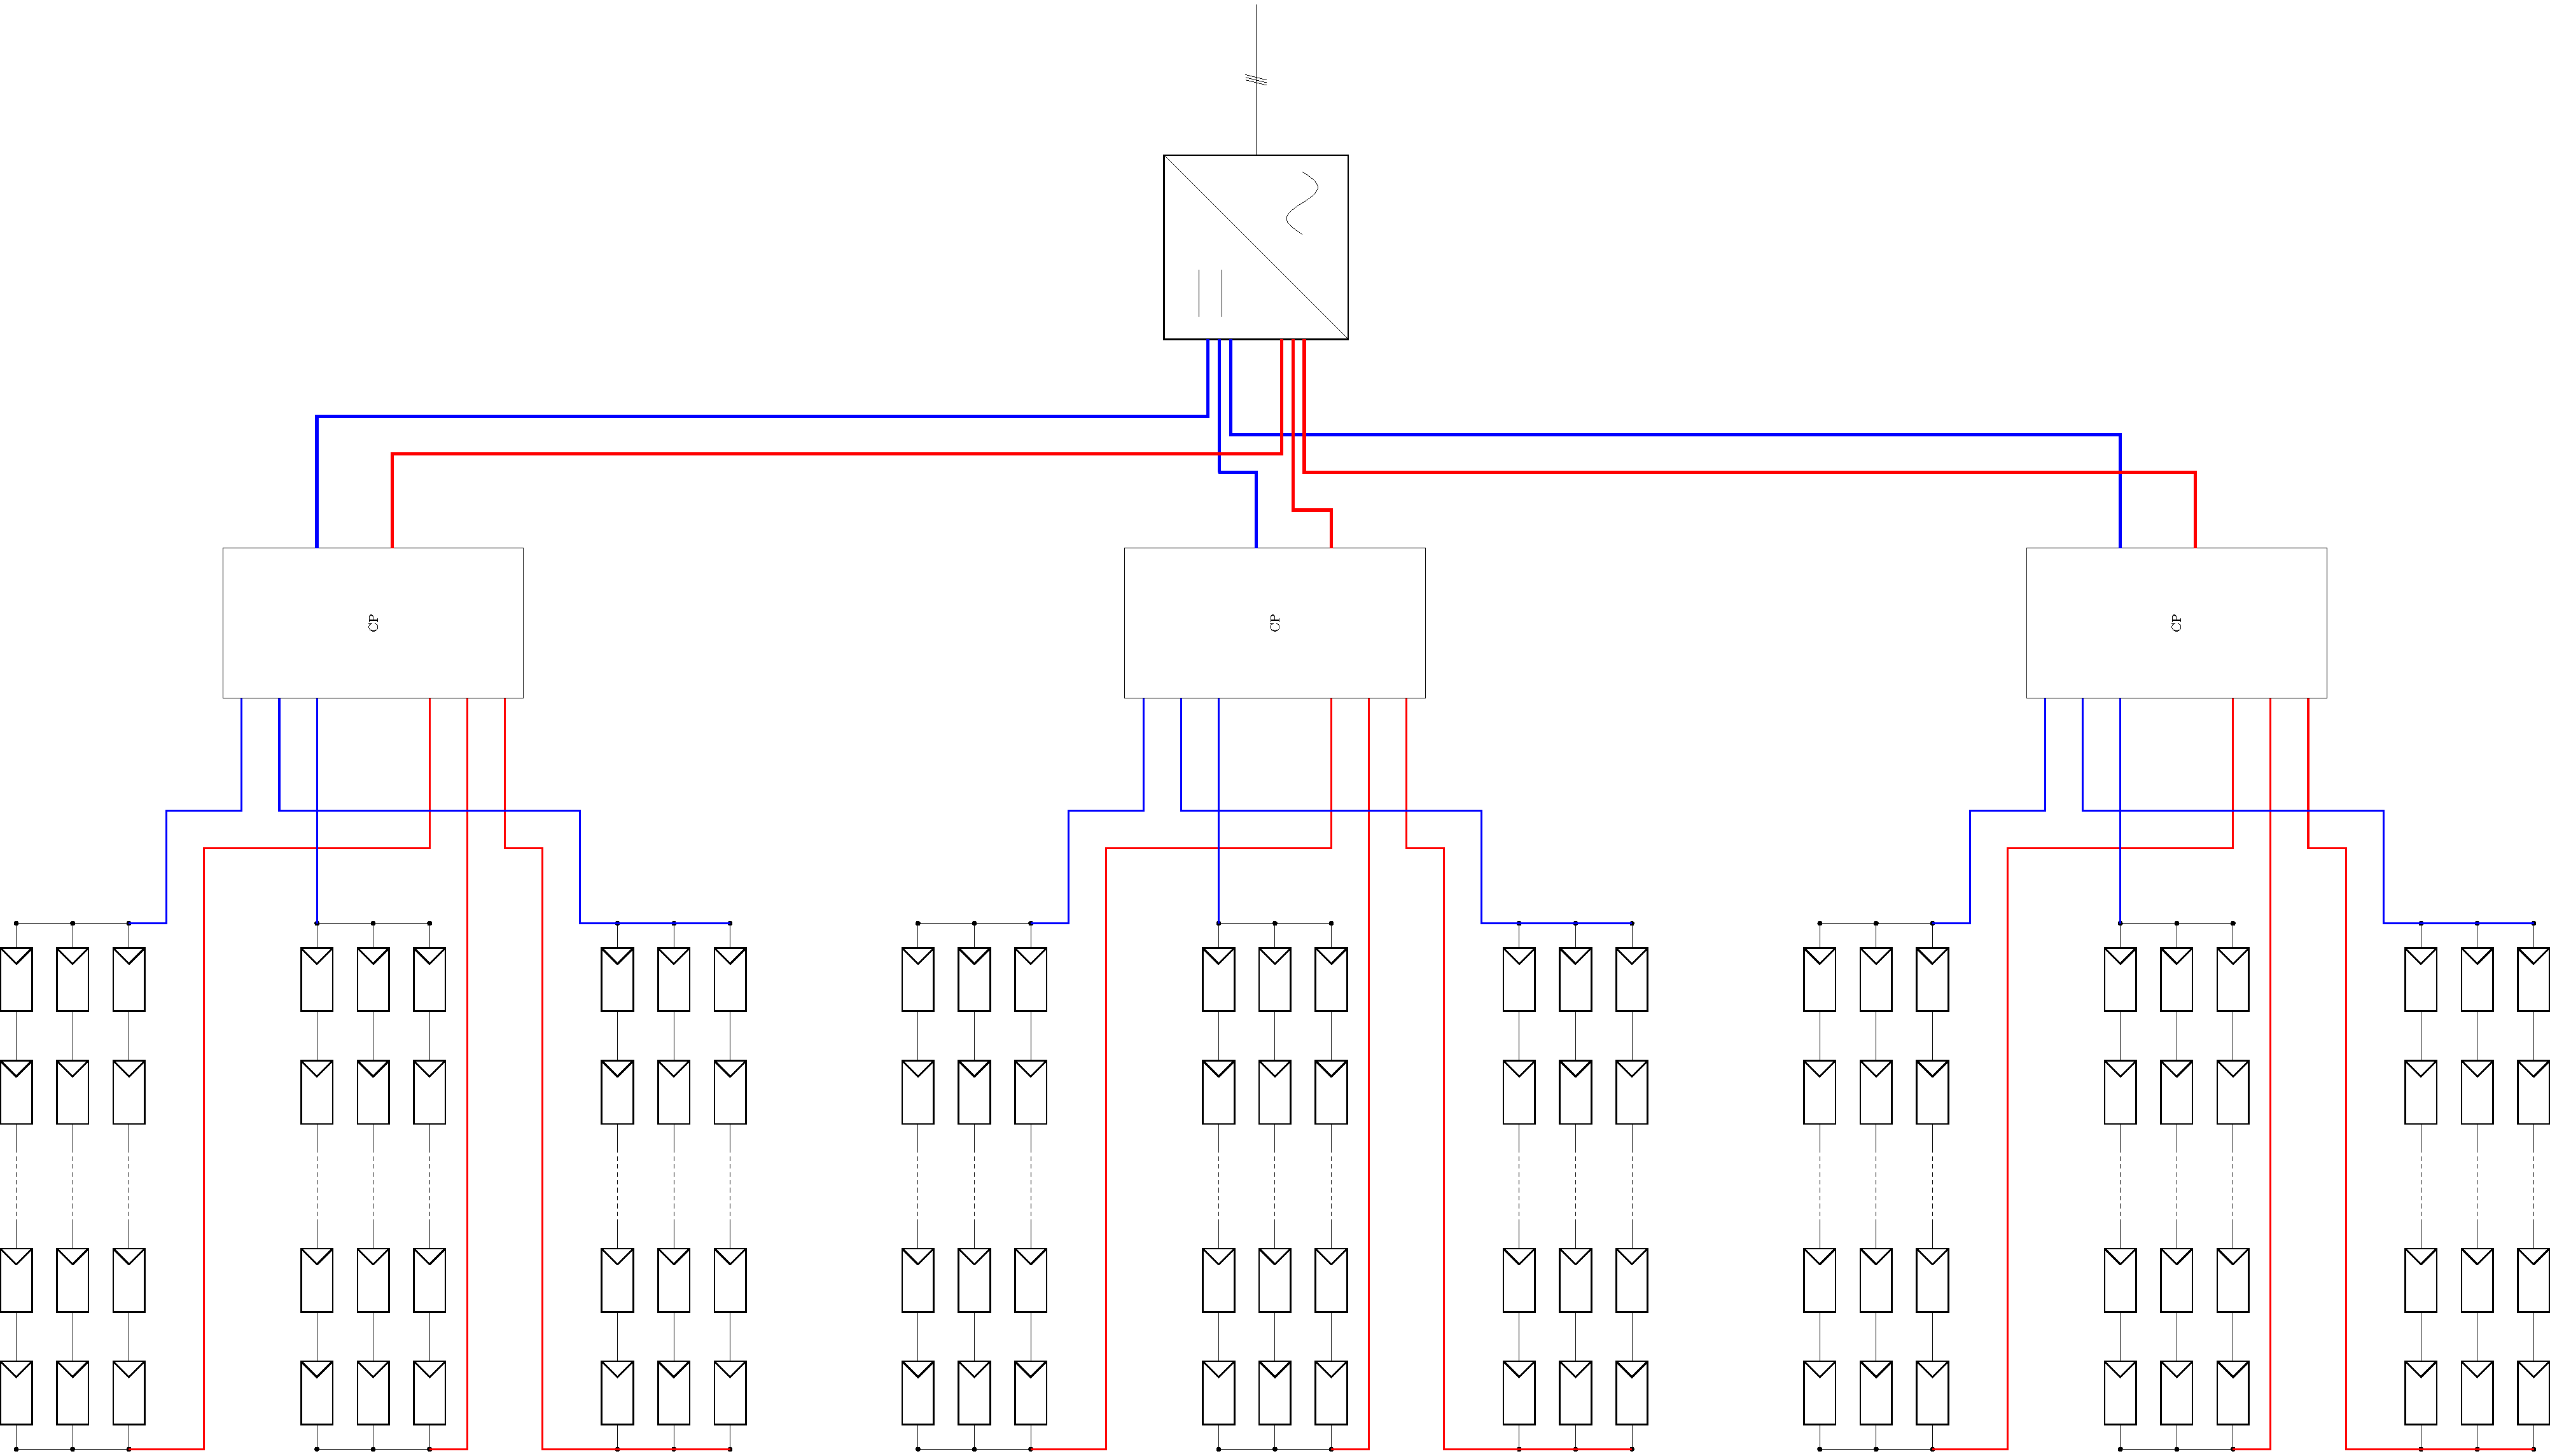
\includegraphics[width=\textwidth]{../figs/CableadoCentral.pdf}
\end{center}
\end{frame}

\begin{frame}[label={sec:orgbb8bf81}]{Características básicas}
\begin{itemize}
\item Criterio de caída de tensión.

\item Comprobar intensidad máxima admisible.

\item En sistemas de gran tamaño reducir bucles.
\end{itemize}
\end{frame}

\begin{frame}[label={sec:org89b690d}]{Criterio de Caída de Tensión}
\begin{itemize}
\item En primer lugar se calculan las secciones mediante el criterio de caida de tensión (RBT ITC-BT-07):
\end{itemize}
\begin{align*}
    S_{dc} &=  \frac{2 \cdot L_{dc}\cdot I_{dc}}{\gamma_\theta \cdot \Delta V_{dc}}\\
    S_{1ac} &=  \frac{2\cdot L_{1ac}\cdot I_{1ac}}{\gamma_\theta \cdot \Delta V_{1ac}}\\
    S_{3ac} &= \frac{\sqrt{3} \cdot L_{3ac}\cdot I_{3ac}}{\gamma_\theta \cdot \Delta V_{3ac}}
  \end{align*}

\begin{itemize}
\item La conductividad del cable, \(\gamma_\theta\), depende del material y de la
temperatura de operación:

\begin{center}
\begin{tabular}{lll}
Material & \(T = \qty{20}{\celsius}\) & \(T = \qty{70}{\celsius}\)\\[0pt]
\hline
Cobre & \(\gamma_{\qty{20}{\degree}} = \qty{58}{\meter\per\ohm\per\milli\meter\squared}\) & \(\gamma_{\qty{70}{\degree}} = \qty{48,47}{\meter\per\ohm\per\milli\meter\squared}\)\\[0pt]
Aluminio & \(\gamma_{\qty{20}{\degree}} = \qty{35,71}{\meter\per\ohm\per\milli\meter\squared}\) & \(\gamma_{\qty{70}{\degree}} = \qty{29,67}{\meter\per\ohm\per\milli\meter\squared}\)\\[0pt]
\end{tabular}
\end{center}
\end{itemize}
\end{frame}

\begin{frame}[label={sec:org1e89967}]{Criterio de Caída de Tensión}
\begin{itemize}
\item Según el apartado 5 de la ITC-BT-40, se exige una caída máxima de
tensión \(\qty{1.5}{\percent}\) de la tensión nominal.

\item Para aplicar correctamente este porcentaje es importante caer en la
cuenta de que \alert{cada zona (DC y AC) tiene su propia tensión nominal}.

\item Cuando un circuito (en DC o AC) está dividido en varios tramos (por
ejemplo, por el uso de cajas de paralelos), la caída de tensión
total del circuito es la suma de las respectivas caídas en cada uno
de los tramos.
\end{itemize}
\end{frame}

\begin{frame}[label={sec:org03ddf15}]{Cálculo por tramos (DC)}
\begin{itemize}
\item Al existir dos tramos y una única condición existe un grado de libertad que permite fijar la sección de uno de los tramos u optimizar el volumen total de conductor empleado.

\item La fracción de caída de tensión en el tramo de la caja al inversor es:  
\begin{equation*}
  \frac{\Delta U_{inv}}{\Delta U}= \frac{1}{1+\sqrt{\frac{\sum_{i=1}^nL_{i}^2
        \cdot I_{i}}{L_{inv}^2 \cdot I_{inv}}}}
\end{equation*}

\begin{itemize}
\item \(\Delta U\) la caída de tensión admisible en el circuito,

\item \(\Delta U_{inv}\) la caída en el tramo desde una caja de paralelos hasta la entrada del inversor,

\item \(L_i\) la longitud de cableado desde el generador hasta la caja de paralelos,

\item \(I_i\) la corriente que circula desde el generador hasta la caja de paralelos,

\item \(L_{inv}\) la longitud de cableado desde la caja hasta el inversor,

\item \(I_{inv}\) la corriente desde la caja hasta el inversor.
\end{itemize}
\end{itemize}
\end{frame}

\begin{frame}[label={sec:org9c623c1}]{Ejemplo de cálculo por tramos (DC)}
En una instalación se agrupan en una caja de paralelos las salidas los generadores ubicados en 20 seguidores, cada uno de ellos con \(\qty{30}{\ampere}\). Esta caja de paralelos está ubicada a \(\qty{200}{\meter}\) del inversor y a \(\qty{30}{\meter}\) de todos los seguidores.
\begin{align*}
  \frac{\Delta U_{inv}}{\Delta U} &= \frac{1}{1+\sqrt{\frac{\sum_{i=1}^nL_{i}^2
                                    \cdot I_{i}}{L_{inv}^2 \cdot I_{inv}}}} = \\
                                  &=\frac{1}{1 + \sqrt{\frac{20 \cdot 30^2 \cdot 30}{200^2 \cdot 600 }}} = \\
                                  &= \num{0.87}
\end{align*}
Si la tensión nominal de los generadores es de \(\qty{500}{\volt}\), este resultado implica que la sección del tramo de la caja de paralelos al inversor se diseñará con una caída de tensión de \(\num{0.87} \cdot \num{1.5} \cdot 500 /100 = \qty{6.525}{\volt}\). El tramo desde los generadores hasta la caja de paralelos se diseñará con una caída de tensión de \((1 - \num{0.87}) \cdot \num{1.5} \cdot 500 /100 = \qty{0.975}{\volt}\).
\end{frame}

\begin{frame}[label={sec:orgb7ac8b9}]{Cálculo AC}
\begin{block}{Ejemplo}
\begin{itemize}
\item En una instalación que conduce \(\qty{75}{\ampere}\) a la salida de un
inversor trifásico, situado éste a \(\qty{100}{\meter}\) de la conexión
a red, se deberá utilizar un cable de sección (suponiendo cobre y teniendo en cuenta
que \(\gamma_{70} = \qty{48}{\meter\per\ohm\per\milli\meter\squared}\)):
\end{itemize}


\[
  S=\frac{\sqrt{3} \cdot 100 \cdot 75}{48 \cdot \qty{1.5}{\percent}\cdot400}=\qty{45.46}{\milli\meter\squared}
\]

\begin{itemize}
\item Dado que la sección de los cables está normalizada, se deberá optar
por la sección inmediatamente superior, y por tanto la conexión del
inversor a la red se realizará con tres cables de sección
\(S=\qty{50}{\milli\meter\squared}\).
\end{itemize}
\end{block}
\end{frame}

\begin{frame}[label={sec:org3bc434b}]{Intensidad Máxima Admisible}
\begin{itemize}
\item Con este resultado, es necesario comprobar que la intensidad de diseño es inferior a la intensidad máxima admisible del cable para sus condiciones de servicio, según las tablas de la ITC-BT-07.

\item No obstante, las secciones que resultan del criterio de caída de tensión aplicado a los sistemas fotovoltaicos habitualmente son sobradamente capaces de conducir la corriente del sistema.
\end{itemize}
\end{frame}

\begin{frame}[label={sec:orgcf33da3}]{Continua vs. Alterna}
Suponiendo que en una planta con varios inversores trifásicos existe la
posibilidad de ubicar los inversores debajo del generador FV
(\emph{distribución en alterna}) o en un centro específico junto al punto de
conexión a red (\emph{distribución en continua}), \alert{¿cuál es la tensión de
trabajo en continua que permite optar por una distribución en continua?}

Se puede demostrar que para tensiones de generador \(V_{mpp} \geq
\qty{475}{\volt}\), la distribución en continua es preferible a la
distribución en alterna desde el punto de vista de masa de conductor
necesario.
\end{frame}


\begin{frame}[label={sec:org034d017}]{Estrategia de Cableado}
\begin{block}{Secuencial (\emph{daisy chain wiring})}
\begin{center}
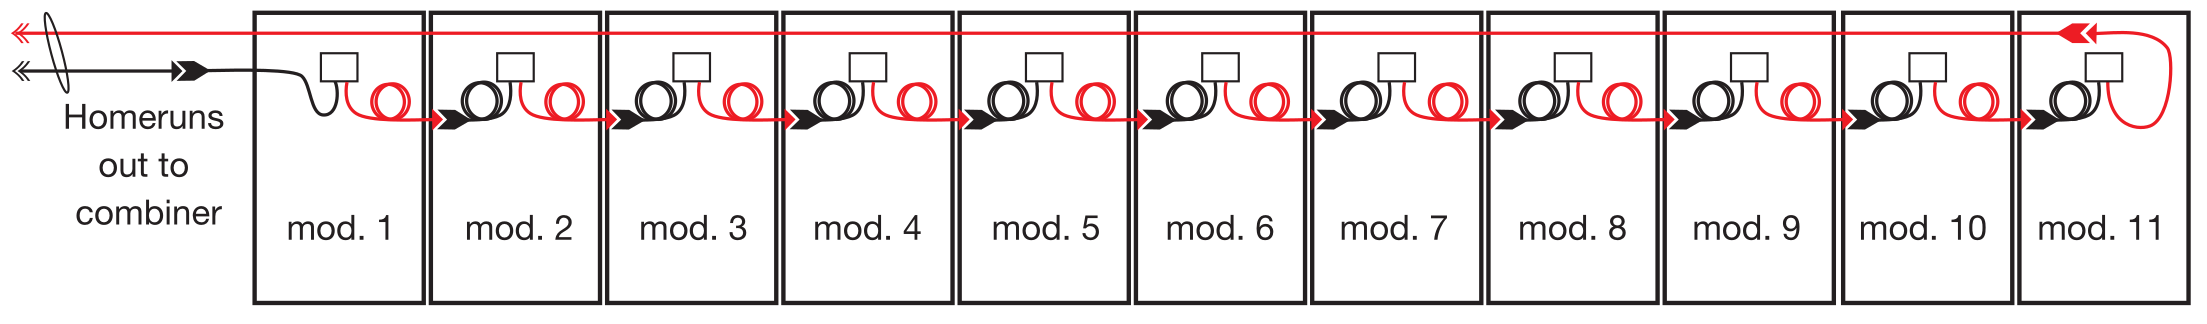
\includegraphics[width=\textwidth]{../figs/DaisyChainWiring.png}
\end{center}

\begin{itemize}
\item Es el modo habitual (todos los instaladores lo conocen).
\item Requiere cable de retorno.
\item El cable sobrante entre módulos debe quedar bien sujeto.
\item Puede requerir más tiempo de instalación.
\end{itemize}
\end{block}
\end{frame}

\begin{frame}[label={sec:org84c0569}]{Estrategia de Cableado}
\begin{block}{Salteado (\emph{leapfrog wiring})}
\begin{center}
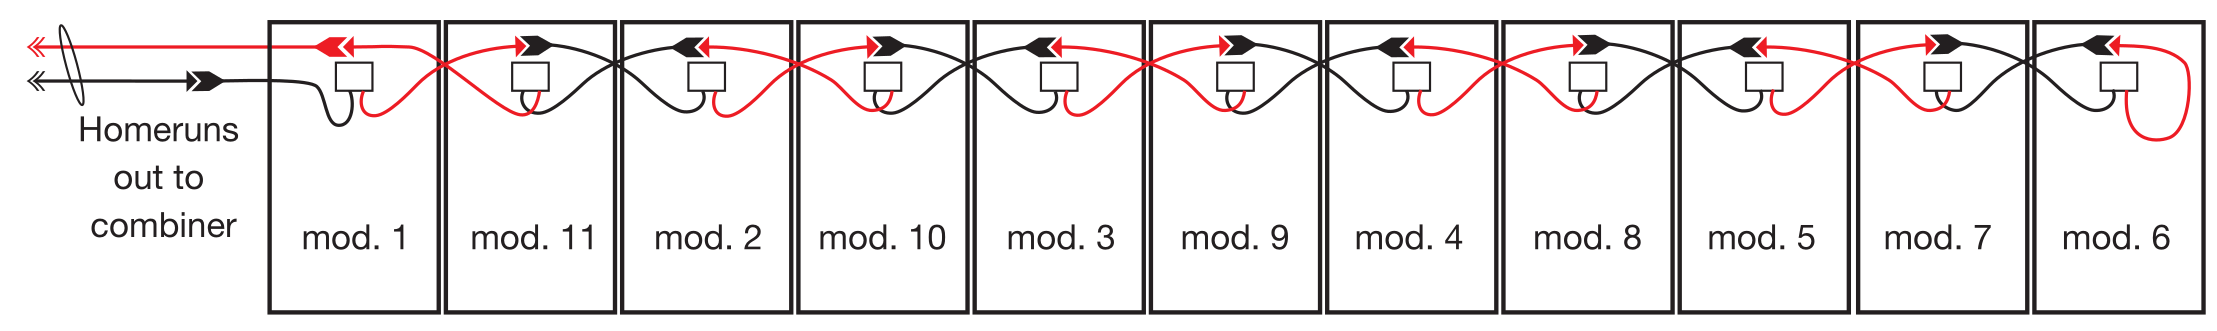
\includegraphics[width=\textwidth]{../figs/LeapfrogWiring.png}
\end{center}

\begin{itemize}
\item No requiere cable de retorno.
\item Reduce bucles electromagnéticos.
\item Hay que comprobar que la longitud del cable del módulo es suficiente.
\item Hay menos cable sobrante entre módulos.
\item Puede requerir menos tiempo de instalación.
\end{itemize}
\end{block}
\end{frame}
\end{document}
